%!TEX root = main.tex

\section{Exercises}

\begin{problem}[Basic]\cite[p.249 \#1]{gautschi2011numerical}
The following sequences all converge to zero. 
\begin{align*}
v_n &= n^{-10} &w_n &= 10^{-n} &x_n &=10^{-n^2} &y_n &=n^{10}3^{-n} &z_n &=10^{-3\cdot 2^n}
\end{align*}
Indicate the type of convergence (See Appendix \ref{appendix:convergence}).  
\end{problem}

\begin{problem}[Advanced]\cite[p.249 \#4]{gautschi2011numerical}
Give an example of a positive sequence $\{ \varepsilon_n \}_{n\in\field{N}}$ converging to zero in such a way that $\lim_n \frac{\varepsilon_{n+1}}{\varepsilon_n^p} = 0$ for some $p>1$, but not converging to zero with any order $q > p$.
\end{problem}

\begin{problem}[Basic]
Find an example of a function $f\colon \field{R} \to \field{R}$ (different from the function in Example \ref{example:NewtonRaphsonloop}) with a unique root at $x=0$ for which the Newton-Raphson sequence is a loop no matter the initial guess $x_0\neq 0$: $x_{2n}=x_0$, $x_{2n+1}=-x_0$ for all $n \in \field{N}$.  Bonus points is your function is trigonometric.
\end{problem}

\begin{problem}[Intermediate]\cite[p.251 \#14]{gautschi2011numerical}
Consider the equation 
\begin{equation*}
x = \cos x.
\end{equation*}
\begin{enumerate}
	\item Show graphically that there exists a unique positive root $x^\star$.  Indicate approximately where it is located.
	\item Show that Newton's method applied to $f(x) = x-\cos x$ converges for any initial guess $x_0 \in \big[0,\frac{\pi}{2}\big]$.
\end{enumerate}
\end{problem}

\begin{problem}[Intermediate]\cite[p.251 \#16]{gautschi2011numerical}
Consider the equation 
\begin{equation*}
\tan x + \lambda x = 0, \quad (0 < \lambda < 1).
\end{equation*}
\begin{enumerate}
	\item Show graphically, as simply as possible, that there is exactly one root $x^\star$ in the interval $\big[ \frac{1}{2}\pi, \pi\big]$.
	\item Does Newton's method converge to the root $x^\star \in \big[ \frac{1}{2}\pi, \pi\big]$ if the initial approximation is taken to be $x_0 = \pi$?  Justify your answer.
\end{enumerate}
\end{problem}

\begin{problem}[Intermediate]\cite[p.252 \#17]{gautschi2011numerical}
Consider the equation 
\begin{equation*}
f(x) = \log^2 x - x -1, (x > 0).
\end{equation*} 
\begin{enumerate}
	\item Graphical considerations suggest that there is exactly one positive root $x^\star$, and that $0 <x^\star < 1$.  Prove this.
	\item What is the largest positive $0<x_0\leq 1$ such that Newton's method started at $x_0$ converges to $x^\star$?
\end{enumerate}
\end{problem}

\begin{problem}[Advanced]\cite[p.252 \#18]{gautschi2011numerical}
Consider Kepler's equation
\begin{equation*}
f(x) = x -a \sin x - b, \quad 0 <\abs{a}<1, \quad b \in \field{R}
\end{equation*}
where $a, b$ are parameters.
\begin{enumerate}
	\item Show that for each $a,b$ there is exactly one real root $x^\star = x^\star(a,b)$ that satisfies
	\begin{equation*}
	b-\abs{a} \leq x^\star(a,b) \leq b+\abs{a}
	\end{equation*} 
	\item Let $m \in \field{N}$ satisfy $m\pi < b < (m+1)\pi$.  Show that Newton's method with starting value
	\begin{equation*}
	x_0 = \begin{cases}
	(m+1)\pi &\text{if }(-1)^ma >0 \\
	m\pi &\text{otherwise}
	\end{cases}
	\end{equation*}
	is guaranteed to converge (monotonically) to $x^\star(a,b)$.
\end{enumerate}
\end{problem}

\begin{problem}[Basic]
Consider the two equivalent equations
\begin{align}
x\log x -1 &= 0, \label{eq:GaustchiLog1} \\
\log x - \frac{1}{x} &= 0. \label{eq:GaustchiLog2}
\end{align}
\begin{enumerate}
	\item Show that there is exactly one positive root and find a rough interval containing it.
	\item For both \eqref{eq:GaustchiLog1} and \eqref{eq:GaustchiLog2}, determine the largest interval on which Newton's method converges. \newline \textbf{Hint: } Investigate the convexity of the functions involved.
\end{enumerate}
\end{problem}

\begin{problem}[CAS]
Design a process in \texttt{desmos.com} to test the search for critical points given by the recursion formulas produced by Newton's method.
\begin{figure}[ht!]
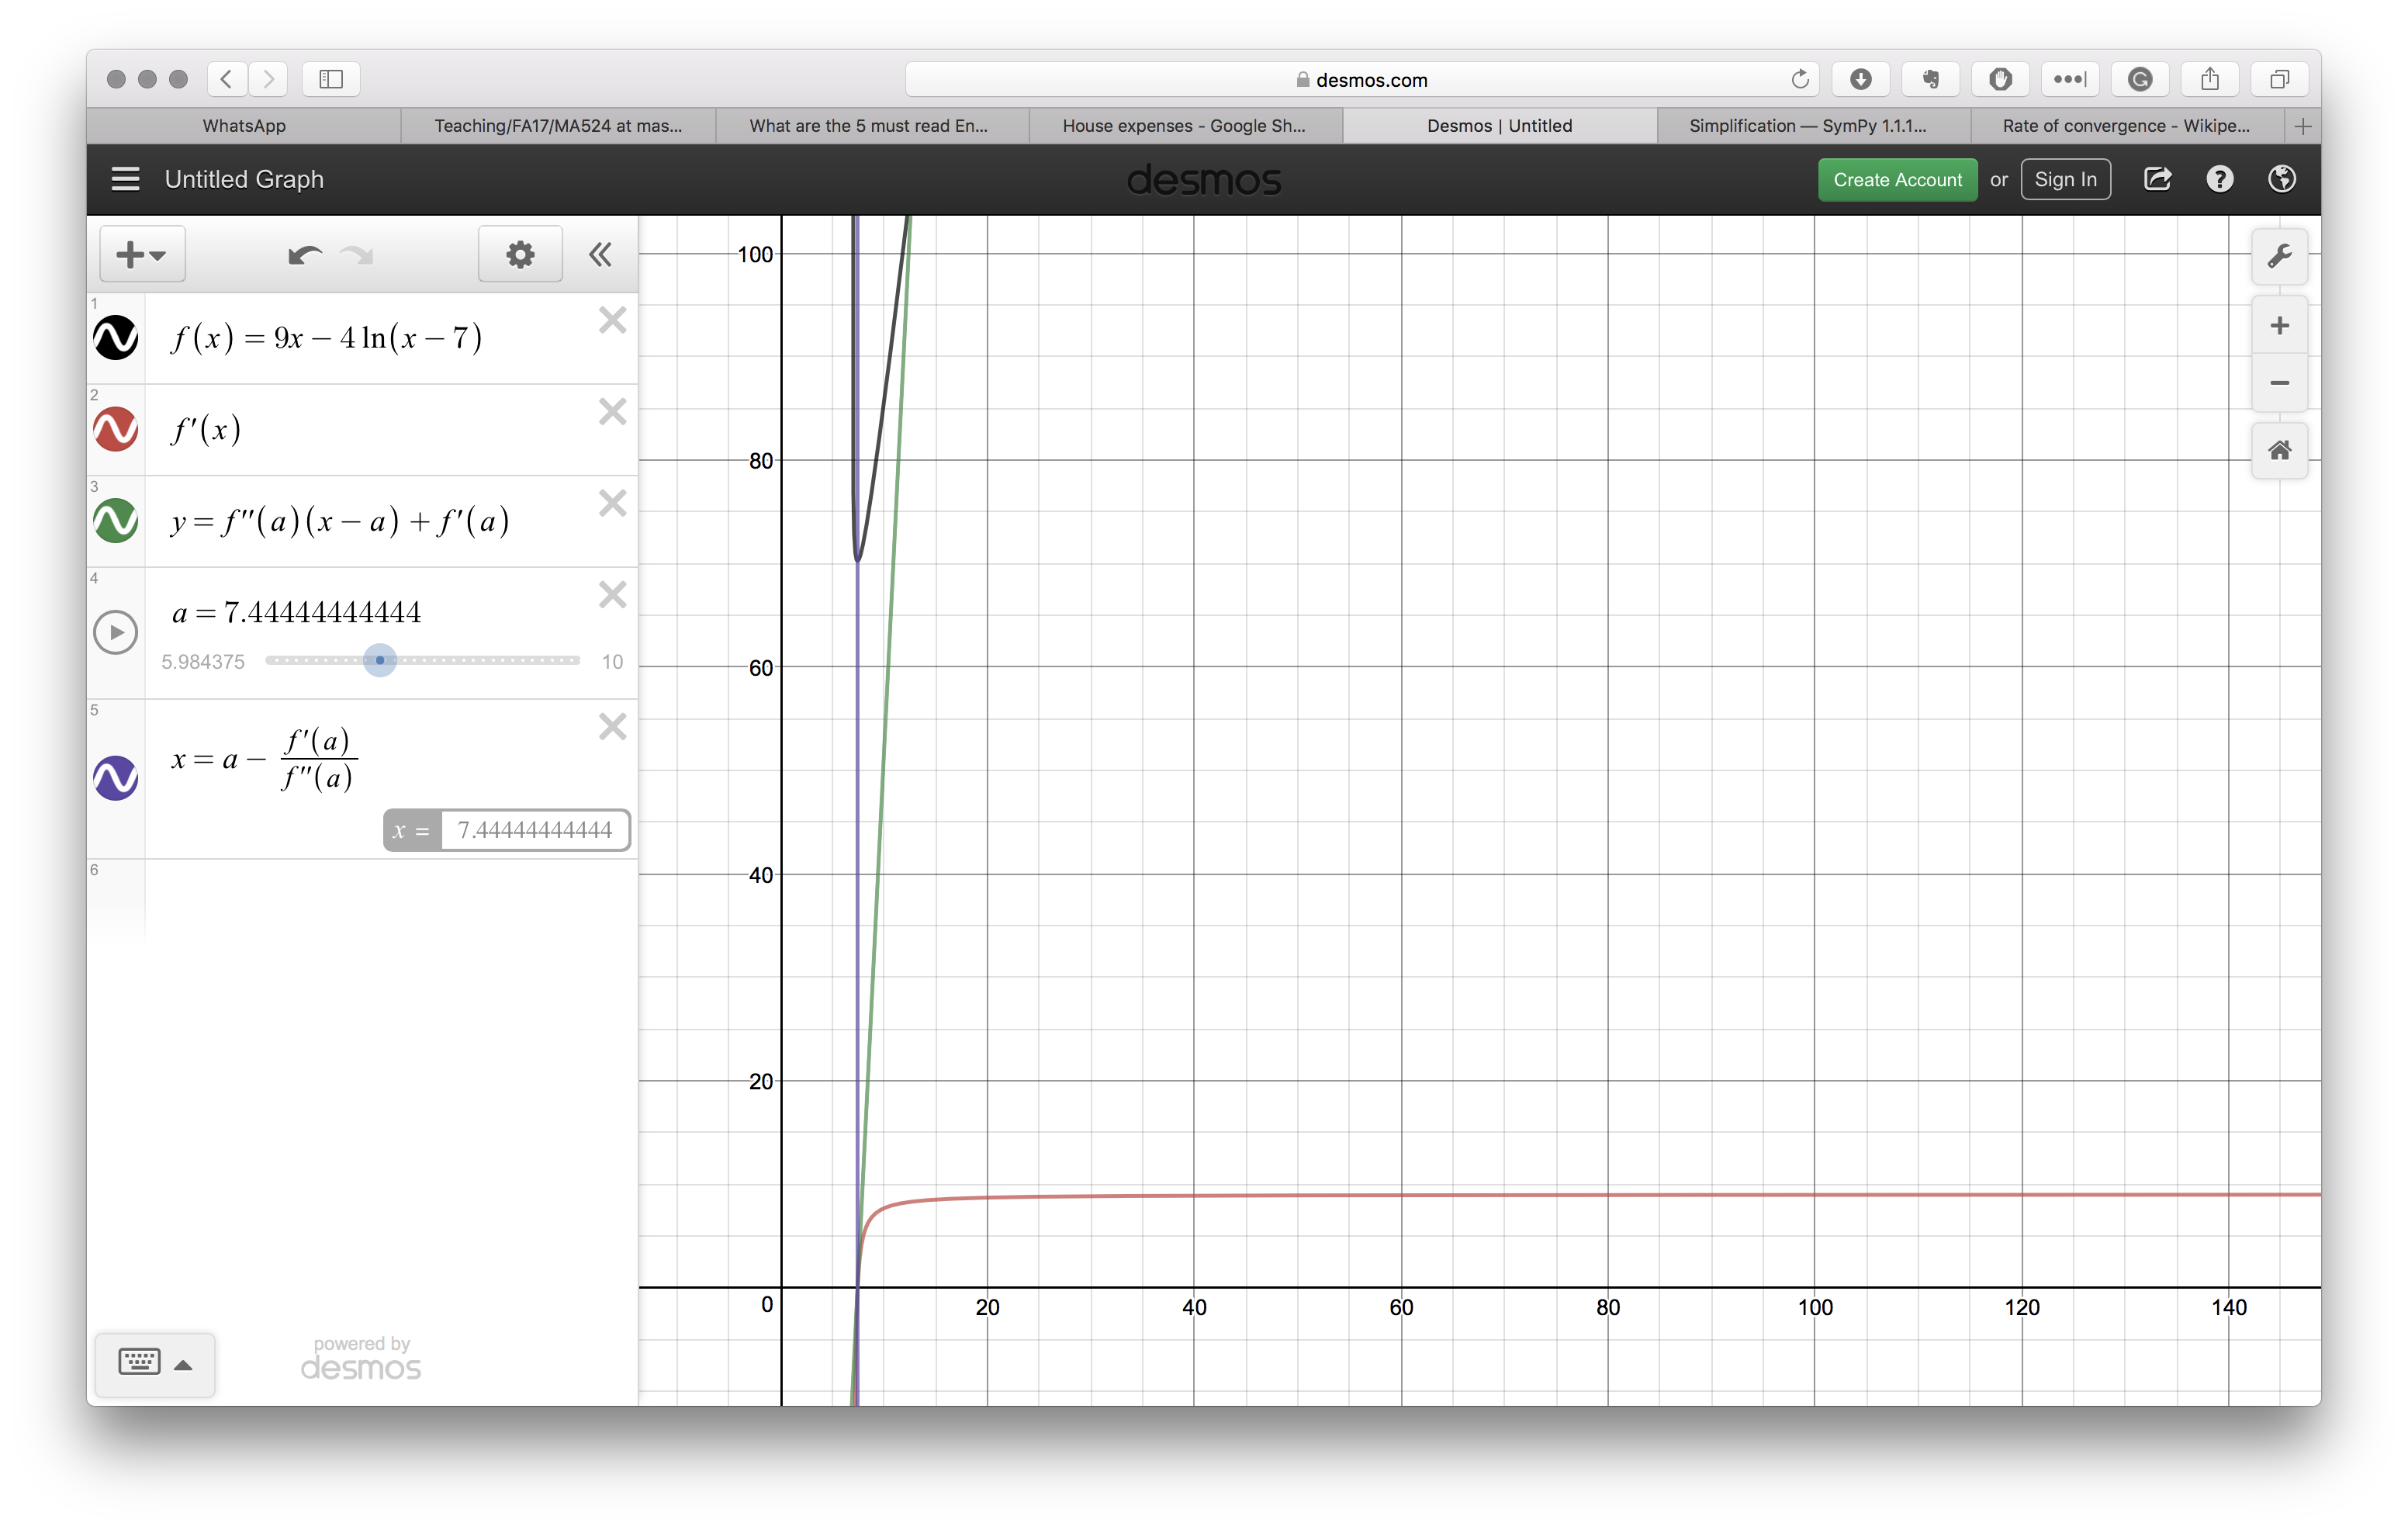
\includegraphics[width=\linewidth]{desmos.png}
\caption{Newton method in \texttt{desmos.com}}
\label{figure:desmosNewton}
\end{figure}
\end{problem}

\begin{problem}[CAS]\label{problem:CASNewton}
In a computer language or CAS of your choice, design a script that gathers 
\begin{itemize}
\item the expression of a generic real-valued function $f\colon \field{R}^d \to \field{R}$, 
\item the gradient $\gradient{f}$ of that function,
\item an initial guess $\x_0 \in \field{R}^d$, 
\item a number $N$ of steps,
\end{itemize}
and produces the first $N+1$ terms of the Newton sequence to approximate a root of $f$.
\end{problem}

\begin{problem}[CAS]
Use script you wrote in Problem \ref{problem:CASNewton} to produce a table and a visual representation for the numerical solution of the following equations, with the given initial guesses:
\begin{enumerate}
\item $f(x) = \sin x$, with $x_0=0.5$, 5 steps.
\item $f(x) = \sin x$, with $x=3$, enough steps to obtain accurately the first 16 correct decimal places of $\pi$.
\item $f(x) = -1+\log x$, with $x=2$, enough steps to obtain accurately the first 16 correct decimal places of $e$.
\end{enumerate}
\end{problem}

\begin{problem}[CAS]
The objective of this problem is to use Newton's method to find an approximation to the golden ratio $\phi=\frac{1}{2}(1+\sqrt{5})$ accurate to the first 16 decimal places.  Find first an appropriate polynomial $p(x)$ with integer coefficients for which $\phi$ is a root.  Employ the script you wrote in Problem \ref{problem:CASNewton}, a good initial guess, and enough steps to guarantee the required result.
\end{problem}

\begin{problem}[Intermediate|CAS]
Consider the function 
\begin{equation*}
f(x) = 9x -4\log(x-7).
\end{equation*}
We wish to study the behavior of Newton-Raphson to find approximations to the critical points of this function.
\begin{enumerate}
	\item Find the domain $D$ of $f$.
	\item Find the global minimum of $f$ analytically.
	\item Compute an exact formula for the Newton-Raphson iterate $x_{n+1}$ for an initial guess $x_0 \in D$.
	\item Compute five iterations of the Newton-Raphson method starting at each of the following initial guesses:
	\begin{enumerate}
		\item $x_0 = 7.4$.
		\item $x_0 = 7.2$.
		\item $x_0 = 7.01$.
		\item $x_0 = 7.8$.
		\item $x_0 = 7.88$.
	\end{enumerate}
	\item Prove that the Newton-Raphson method converges to the optimal solution for any initial guess $x_0 \in (7,7.8888)$.
	\item What is the behavior of the Newton-Raphson method if the initial guess is not in the interval $(7,7.8888)$?
\end{enumerate}
\end{problem}

\begin{problem}[Intermediate|CAS]
Consider the function 
\begin{equation*}
f(x) = 6x -4\log(x-2) -3\log(25-x).
\end{equation*}
We wish to study the behavior of Newton-Raphson to find approximations to the critical points of this function.
\begin{enumerate}
	\item Find the domain $D$ of $f$.
	\item Find the global minimum of $f$ analytically. 
	\item Compute an exact formula for the Newton-Raphson iterate $x_{n+1}$ for an initial guess $x_0 \in D$.
	\item Compute five iterations of the Newton-Raphson method starting at each of the following initial guesses:
	\begin{enumerate}
		\item $x_0 = 2.6$.
		\item $x_0 = 2.7$.
		\item $x_0 = 2.4$.
		\item $x_0 = 2.8$.
		\item $x_0 = 3$.
	\end{enumerate}
	\item Prove that the Newton-Raphson method converges to the optimal solution for any initial guess $x_0 \in (2,3.05)$.
	\item What is the behavior of the Newton-Raphson method if the initial guess is not in the interval $(2,3.05)$?
\end{enumerate}
\end{problem}

\begin{problem}[Advanced]\cite[p.91 \#1.4.1]{bertsekas1999nonlinear}
The purpose of this exercise is to show that Newton's method is unaffected by linear scaling of the variables.  Consider a linear invertible transformation of variables $\x=\boldsymbol{A}\y$.  Write Newton's method in the space of the variables $\y$ and show that it generates the sequence $\y_n = \boldsymbol{A}^{-1}\x_n$, where $\{ \x_n \}_{n \in \field{N}}$ is the sequence generated by Newton's method in the space of variables $\x$.\
\end{problem}

\begin{problem}[Advanced]
Prove Theorems \ref{theorem:SteepestDescentDescends}, and \ref{theorem:SteepestDescentConvergesToCritical}.
\end{problem}
